\documentclass{standalone}
\usepackage{tikz}

\usepackage{color}

\usetikzlibrary{arrows.meta}
\usetikzlibrary{calc}
\usetikzlibrary{shapes}
\usetikzlibrary{bending}
\usetikzlibrary{patterns}

\usepackage{gensymb}

\usepackage{pgfplots}
\usepackage{amsmath}


\begin{document}
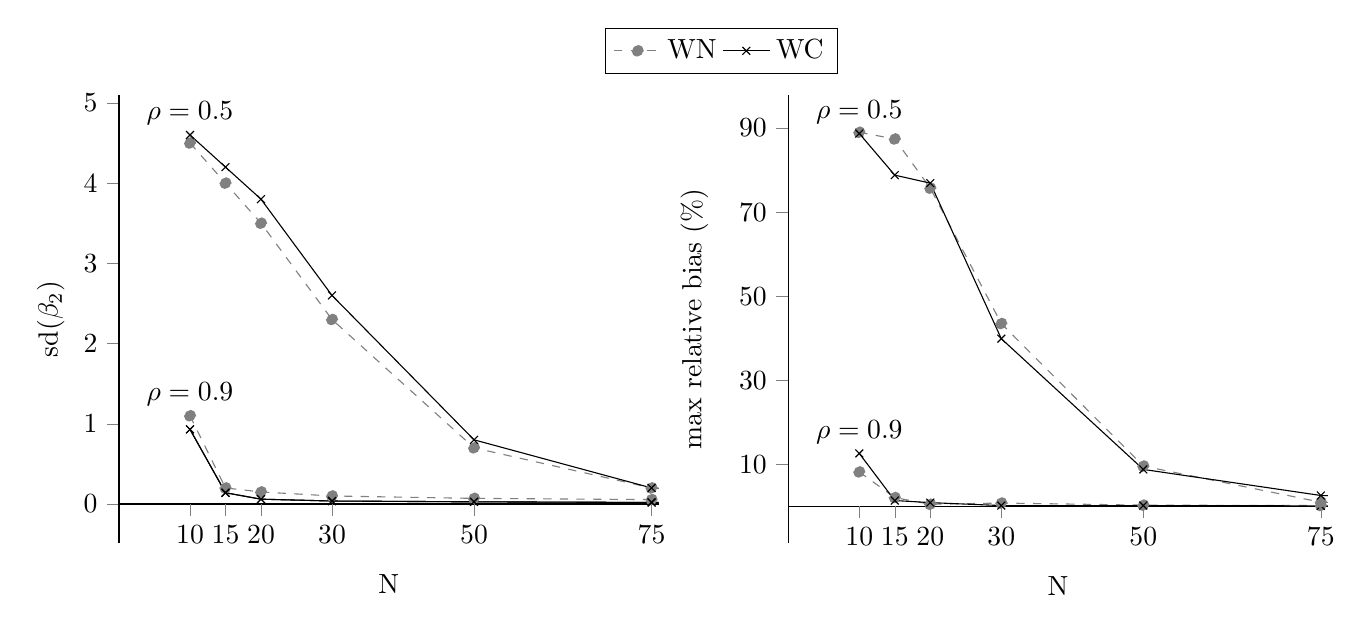
\begin{tikzpicture}[
	scale=1,
	]	
	
	%WN sds
	\begin{axis}[
	axis on top=true,
	%xshift= 6cm,
	scale=1,
	%width=15cm,
	axis x line*=middle , axis y line*=left,
	xtick=\empty,
	%ytick=\empty,
	%extra y ticks = {0.02, 0.05, 0.07, 0.1, 0.14},
	%extra y tick labels = {0.02, 0.05,0.07, 0.10, 0.14},
	ytick align = outside,
	xtick align = outside,
	xlabel = {N},
	ylabel = sd($\beta_2$),
	extra x ticks = {10, 15, 20, 30, 50, 75,100},
	xlabel near ticks,
	ymax=5.1,
	xmin=0, xmax=76,
	legend style ={at={(0.90,1.15)}, 
		anchor=north west, draw=black, 
		fill=white, legend columns=-1}]
	

	\addplot[mark=*, color=gray, dashed]    coordinates {(10,1.1)(15, 0.2)(20, 0.15)(30,0.10)(50,0.07)(75,0.055)(100,0)} node[pos=0] (rho) {};
	\node [above] at (rho) {$\rho=0.9$}; %rho=0.9
	\addlegendentry{WN};
	\addplot[mark=x, color=black]   coordinates {(10,0.93)(15, 0.14)(20, 0.06)(30,0.037)(50,0.027)(75,0.019)(100,0.016)};  
	\addlegendentry{WC};
	
	\addplot[mark=*, color=gray, dashed]    coordinates {(10,4.5)(15, 4.0)(20, 3.5)(30,2.3)(50,0.7)(75,0.2)(100,0)}; 
	\addplot[mark=x, color=black]   coordinates {(10,4.6)(15, 4.2)(20, 3.8)(30,2.6)(50,0.8)(75,0.2)(100,0.12)} node[pos=0] (rho) {};
	\node [above] at (rho) {$\rho=0.5$}; %rho=0.5
	
	\addplot[mark=x, color=black]   coordinates {(10,0.93)(15, 0.14)(20, 0.06)(30,0.037)(50,0.027)(75,0.019)(100,0.016)};   

	
\end{axis}
	
\begin{axis}[
	axis on top=true,
	xshift= 8.5cm,
	scale=1,
	%width=15cm,
	axis x line*=middle , axis y line*=left,
	xtick=\empty,
	ytick=\empty,
	extra y ticks = {10, 30, 50, 70, 90},
	%extra y tick labels = {0.02, 0.05,0.07, 0.10, 0.14},
	ytick align = outside,
	xtick align = outside,
	xlabel = {N},
	ylabel = max relative bias (\%),
	extra x ticks = {10, 15, 20, 30, 50, 75,100},
	xlabel near ticks,
	%ymin=0, ymax=2.0,
	xmin=0, xmax=76]
	

	\addplot[mark=*, color=gray, dashed]    coordinates {(10,8.2)(15, 2.1)(20, 0.5)(30,0.8)(50,0.3)(75,0.2)(100,0)} ;
	\addplot[mark=x, color=black]   coordinates {(10,12.6)(15, 1.4)(20, 0.9)(30,0.2)(50,0.2)(75,0.13)(100,0.14)} node[pos=0] (rho) {};
	\node [above] at (rho) {$\rho=0.9$}; %rho=0.9  
	
	\addplot[mark=*, color=gray, dashed]    coordinates {(10,89.0)(15,87.4)(20, 75.7)(30,43.5)(50,9.6)(75,1.0)(100,0)}; 
	\addplot[mark=x, color=black]   coordinates {(10,88.7)(15,78.8)(20, 76.9)(30,39.9)(50,8.8)(75,2.6)(100,1.3)} node[pos=0] (rho) {};
	\node [above] at (rho) {$\rho=0.5$}; %rho=0.5
	
	\end{axis}
	
	\end{tikzpicture}  
\end{document}